\documentclass[dvipdfmx,18pt]{jsarticle}
\usepackage{graphics}
\usepackage{amsmath}
\usepackage{amssymb}
\usepackage{amsthm}
\usepackage{mathtools}
\usepackage{ascmac}
\usepackage{bm}
\usepackage{url}
\usepackage{txfonts}
\usepackage{color}
\usepackage{tikz}
\usetikzlibrary{calc}
\usetikzlibrary{intersections}

\begin{document}
    \section*{初めに}
    中学数学の中でのやや面倒な単元である濃度と密度について扱う.この2つは根元のところで同じなので,同時に理解したい.この資料は中学生向けではある.しかし,読みにくい場合は両親の助けを借りるように.

    さて,早速だがこの資料で一番大事なテーマをここで示しておく.それは

    {\centering 一部分がわかれば全体の様子がわかる\\}
    というものだ.
    これは科学(理系の勉強)のすべてに共通する大事な発想だ.濃度・密度は一部分を知ることで全体がわかる最も簡単な例になっている.


    次の節から本題に入る.まずは濃度から扱う.

    \section{濃度}
    \subsection{同じしょっぱさ}
    食塩水の濃度を考える問題では,外すことができない大事な条件がある.問題文には書かれていないことが多い.それは,"食塩水は完全に混ざっている"という条件だ.簡単に言うと,食塩水のどの部分を飲んでも同じしょっぱさだということだ.そして,それは大きな食塩水のバケツからいくらコップに食塩水をくんできても同じものになるということでもある(図\ref{tikz_baketu_shokuensui}).

    \begin{figure}[htbp]\centering
        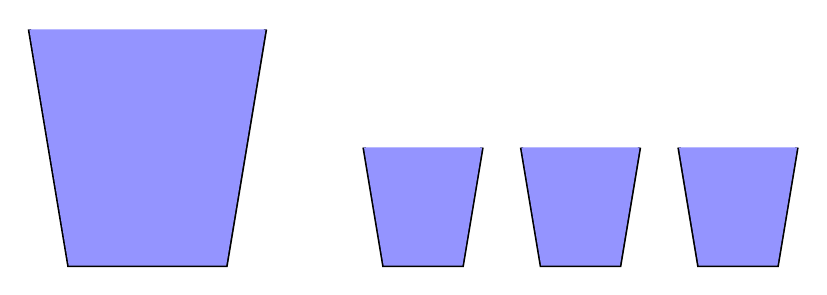
\begin{tikzpicture}\large
            \draw[very thick]($2*(-.25,1.5)$)--(0,0)--($2*(1,0)$)--($2*(1.25,1.5)$);
            \fill[blue!42]($2*(-.25,1.5)$)--(0,0)--($2*(1,0)$)--($2*(1.25,1.5)$);

            \foreach \x in{4,6,8}{
                \draw[very thick](\x -.25,1.5)--(\x,0)--(\x +1,0)--(\x +1.25,1.5);
                \fill[blue!42](\x -.25,1.5)--(\x,0)--(\x +1,0)--(\x +1.25,1.5);
            }

        \end{tikzpicture}
        \caption{大きなバケツから食塩水をとる}
        \label{tikz_baketu_shokuensui}
    \end{figure}

    間違っても図\ref{tikz_baketu_shokuensui_sub}のように,くんだコップによってしょっぱい度合いが変わることはない.

    \begin{figure}[htbp]\centering
        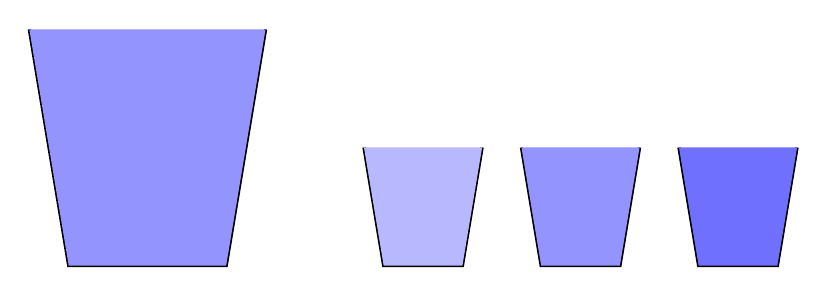
\begin{tikzpicture}\large
            \draw[very thick]($2*(-.25,1.5)$)--(0,0)--($2*(1,0)$)--($2*(1.25,1.5)$);
            \fill[blue!42]($2*(-.25,1.5)$)--(0,0)--($2*(1,0)$)--($2*(1.25,1.5)$);

            \foreach \x in{28,42,56}{
            \draw[very thick](\x/7 -.25,1.5)--(\x/7,0)--(\x/7 +1,0)--(\x/7 +1.25,1.5);
            \fill[blue!\x](\x/7 -.25,1.5)--(\x/7,0)--(\x/7 +1,0)--(\x/7 +1.25,1.5);
            }

        \end{tikzpicture}
        \caption{大きなバケツから食塩水をとる}
        \label{tikz_baketu_shokuensui_sub}
    \end{figure}

    この条件は,コップの様子を知ることができれば,バケツ全体の様子がわかることを示している.つまり,"一部分がわかれば全体のようすがわかる"である.

    \subsection{コップとバケツ}
    前項\footnote{この資料では「濃度」や「同じしょっぱさ」という部分に番号が振ってある.これは節・項を示している.「濃度」節の「同じしょっぱさ」項と理解しよう.つまり,ここでの前項は「同じしょっぱさ」項である.このような書き方は以降も続く.}でバケツの水をコップに取り出すと,コップにバケツの様子が部分として映ることを述べた.これをもっと数学的に考える.

    数学的というのはコップというまちまちな基準\footnote{どんなコップでもいいというのは,数学的ではない.}ではなく,1つの変化しない基準を使うということだ.そこで使うのが \(1\ \mathrm{g}\)という量だ.当然,この量は変化しない.
    そして, \(1\ \mathrm{g}\)というコップに対してバケツに当たるのが水溶液全体ということになる.

    ここまでで,何となくコップとバケツが数学的に何になるのかがわかったが,いまいち関係がつかめない.これは水溶液の様子というのが何なのかを示していないからだ.これは次項で述べる.

    \subsection{水溶液の様子}
    これまでの話で,水溶液の"様子"というのは全体を示すバケツからだけではなく,その一部分のコップからもわかることを述べた.さらに,数学的にはバケツは水溶液全体を,コップが \(1\ \mathrm{g}\)という量であると紹介した.ここでは水溶液の"様子"というものが何なのかを明らかにする.

    結論から述べると,水溶液の"様子"というのは,
    水溶液に溶ける溶質(塩など)の重さ[\(\mathrm{g}\)]のことだ.水溶液を扱う問題で理解が難しいのは,この水溶液の"様子"というものと,"濃度"というものの区別だ.
    次のような関係になっている(図\ref{tikz_yosu_nodo}).

    \begin{figure}[htbp]\centering
        \begin{tikzpicture}
            \node[draw](a) at (0,0){\(1\ \mathrm{cm}^2\)の塩の量:濃度};
            \node[draw](b) at (6,0){全体の塩の量:様子};
            \draw[thick,<->](a)node[above=3mm]{一部分}--node[above]{食塩水の量}(b)node[above=3mm]{全体};
        \end{tikzpicture}
        \caption{"様子"と"濃度"}
        \label{tikz_yosu_nodo}
    \end{figure}

    この関係がわかっていると実際に濃度を計算するときの式に間違いが起きにくい.

    \subsection{濃度の計算}
    ここまでの話を使って,ようやくここで濃度を計算する.
    % 水溶液の濃度を考えるときは食塩水の量や水の量,塩の量はすべてグラムで考える.
    まず図\ref{tikz_baketu_shokuensui}のように全体の水溶液から \(1\ \mathrm{{g}}\)ずつ水溶液を分けてゆくことをイメージする.このとき,コップのしょっぱさはすべて同じなのだから, \(1\ \mathrm{g}\)のコップに入っている塩の量はすべて同じといえる\footnote{同じ量の食塩水で同じしょっぱさなら,塩の量は同じに決まっている.}.つまり,塩だけに注目するとバケツからコップに分けるとは,塩を同じ量で分けるということになる.

    元のバケツをすべてコップに分けると,塩はすべてのコップに同じだけ入ることになる\footnote{ピッタリいかない最後のコップは仕方ない.}.では1つのコップにどれだけの塩が入るかは,元の塩の量をコップの数で割ればいいことがわかる.

    % 元の塩の量はすぐにわかる.さらにコップの数は,バケツに入った食塩水の量であるとわかる.ここから次の式を与えることができる.

    最後に濃度は百分率で表さなければならないので100をかける\footnote{これについては次項で述べる.}ことを忘れなければ,次の式を立てることができる.

    \begin{equation}
        (\text{食塩水の濃度(\%)}) = \frac{(\text{塩の量(g)})}{(\text{食塩水の量(g)})}\times 100
    \end{equation}

    食塩水の量は食塩水の作るときに使う塩の量と,水の量の和ということができるので,次のようにすることもできる.

    \begin{equation}
        (\text{食塩水の濃度(\%)}) = \frac{(\text{塩の量(g)})}{(\text{水の量(g)})+(\text{塩の量(g)})}\times 100
    \end{equation}

    基本的に水溶液の濃度の計算では塩が変わったりすることがあっても上の2つの式を使うだけでよい.

    \subsection{百分率}
    百分率とは,小さな数値に100かけることで見やすい値にする計算方法だ.小さな数値というのも特に0から1までの範囲に入る数値のことだ.それ以上の意味があるわけではない.

    例えば,コインの裏表は2分の1の確率で \(1/2=0.5\)であるが,百分率では
    \[
    0.5\times 100 =50\ \%
    \]
    となる.

    これを濃度でも使う.
    \[
    \frac{(\text{塩の量(g)})}{(\text{食塩水の量(g)})}
    \]
    この値は確実に0から1までの間に入る数なので100をかけて見やすくすることで濃度とする.

    \section{濃度計算の理解}
    ここまでで,水溶液の成り立ちや公式について述べた.ここでそれらをまとめる.
    \subsection{目的}
    まずは濃度を利用する目的だ.もともとの目的はバケツの中にある水溶液に入っている塩の量を求めることだ.これを達成するために,バケツの中身をすべて出していては無駄が多い.そのため,コップ1杯の水溶液に注目して計算することで,塩の量を求めるのだ.

    このとき,水溶液の塩がまんべんなく混ざっていることが,計算をするための条件となっていることに注意しよう.

    \subsection{計算方法}
    バケツの塩をコップに等分するというのが濃度の計算の最も大事な考え方だ.そして,コップというのが \(1\mathrm{g}\)であると考えることで計算が可能になる.バケツの中の水溶液を \(1\mathrm{g}\)のコップに分けるのだから,コップの数は
    \[
       (\text{コップの数})= \frac{\text{(バケツの中の重さ(g))}}{\text{(コップ1杯(g))}}
    \]
    ということになるので,コップ1杯当たりの塩の重さは
    \[
        (\text{コップ1杯の塩の重さ(g)})= \frac{(\text{塩の重さ})}{(\text{バケツの中の重さ(g)})}
    \]
    となる.

    ここまでで濃度といっても問題がないように感じるが,計算結果は必ず0から1の間の小さな数字になってしまう.これでは,どれくらい塩が入っているのかがわかりにくい.そこで100をかけることで百分率として見やすくするのだ.最終的に,濃度の計算は次の式でなされる.
    \begin{equation}
        (\text{濃度})=\frac{(\text{塩の重さ(g)})}{(\text{水溶液全体の重さ(g)})}=\frac{(\text{塩の重さ(g)})}{(\text{水の重さ(g)})+(\text{塩の重さ(g)})}
    \end{equation}


\end{document}
